% vim:spell:spelllang=en
\chapter{Register Allocation\Author{F. Bouchez \andAuthor S. Hack}}
\label{chapter:register_allocation}
\inputpath{part4}{register_allocation}
\inputprogress

{

\newenvironment{important}{%
\bgroup \color{blue!50!black}
  }{
\egroup 
}

%% Local macros for personal use
\newcount\todocount \todocount=0
\def\todo#1{\global\advance\todocount by 1 {\color{blue} {\bf TODO:} #1}}
\newlinechar=`\^^J
\def\endofchapter{\ifnum\todocount>0\immediate\write16{^^JLaTeX Warning: There 
was still TODO macros: \the\todocount.^^J}\fi}


\def\
\def\ac#1{#1}
\def\dom{\preceq}
\def\ssa{SSA\xspace}
\def\maxlive{\ensuremath{\mathrm{Maxlive}}\xspace}
\def\regs{\ensuremath{R}\xspace}
\def\irc{Iterated Register Coalescing\xspace}




Register allocation maps the variables of a program to physical memory locations.
The compiler determines the location for each variable and each program point.
Ideally, as many operations as possible should draw their operands from processor registers without loading them from memory beforehand.
Due to the large latency of the memory hierarchy, register allocation is one of the most important optimizations in a compiler. 
As there is only a small number of registers available in a CPU (with usual values ranging from~8 to~128), it is usually not possible to only use registers, and the task of register allocation is also to decide which variables should be evicted from registers and at which program points to store and load them from memory (spilling).

Furthermore, register allocation has to remove spurious copy operations (copy coalescing) inserted by previous phases in the compilation process, and to deal with allocation restrictions that the instruction set architecture and the run-time system impose (register targeting).
Classical register allocation algorithms address those different issues with either complex and sometimes expensive schemes (usually graph-based), or simpler and faster (but less efficient) algorithms such as linear scan.

The goal of this Chapter is to illustrate how SSA form can help in designing both simpler and faster schemes with similar or even better quality than the most complex existing ones.

\section{Introduction}

Let us first review the basics of register allocation, to help us understand the choices made by graph-based and linear-scan style allocations.

Register allocation is usually performed per procedure. 
In each procedure, a liveness analysis (see Chapter~\ref{chapter:liveness}) determines for each variable the program points where the variable is alive. 
The set of all program points where a variable is alive is called the \emph{live-range} of the variable, and all along this live-range, storage needs to be allocated for that variable, ideally a register. When two variables ``exist'' at the same time, they are conflicting for resources, i.e., they cannot reside in the same location.

This resource conflict of two variables is called \emph{interference} and is usually defined via liveness: 
two variables interfere if (and only if) there exists a program point where they are simultaneously alive, i.e., their live-ranges intersect.%
\footnote{ This definition of interference by liveness is an over-approximation (see Section~\ref{sec:properties_and_flavors:ultimate_interference}), and there are refined definitions that create less interferences (see Chapter~\ref{chapter:alternative_ssa_destruction_algorithm}). 
  However, in this chapter we will restrict ourselves to this definition and assume that two interfering variables cannot be assigned the same register. 
}
It represents the fact that those two variables cannot share the same register.
For instance, in Figure~\ref{fig:ra:linearscan}, variables $a$ and $d$ interfere as $a$ is alive at the definition of $d$.

\subsection{Questions for register allocators}

There are multiple questions that arise at that point that a register allocator has to answer:
\begin{itemize}
  \item Are there enough registers for all my variables? (\emph{spill test})
  \item If yes, how do I choose which register to assign to which variable? (\emph{assignment})
  \item If no, how do I choose which variables to spill to memory? (\emph{spilling})
\end{itemize}

Without going into the details, let us see how linear-scan and graph-based allocators handle these questions.

\paragraph{Linear-scan} The linear-scan principle is to consider that a procedure is a long basic block, and to scan it from top to bottom.
When encountering the definition of a variable (i.e., the beginning of a live-range), we check if some registers are free (\emph{spill test}).
If yes, we pick one to assign the variable to (\emph{assignment}). If no, we choose from the set of currently live variables the one that has the farthest use and spill it (\emph{spilling}).
When we encounter the last use of a variable (i.e., the end of its live-range), we free the register it was assigned to.

\paragraph{Graph-based}
Graph-based allocators, such as the ``Iterated Register Coalescing'' allocator (IRC), represent interferences of variables as an undirected \emph{interference graph}: the nodes are the variables of the program, and two nodes are connected if they interfere.
In this model, two neighbouring nodes must be assigned different registers, so the assignment of variables to registers amounts to \emph{coloring} the graph using at most $R$ colors, the number of registers.\footnote{Hence the terms ``register'' and ``color'' will be used interchangeably in this chapter.}

Here, the allocator will try to color the graph, if it succeeds (\emph{spill test}), then the coloration represents a valid assignment of registers to variables (\emph{assignment}). If not, the allocator will choose some nodes (usually the ones with the highest number of neighbours) and remove them from the graph by storing the corresponding variables in memory (\emph{spilling}).


\paragraph{Comparison}

Linear-scan is a very fast allocator that works directly on the procedure.
In its model, its spill test is exact and its spill minimizes the amount of loads and store.
However, the model itself has a large flaw as procedures generally are not just straight-line code but involve complex flow structures such as if-conditions and loops.
In this model, the live-ranges are artificially longer so produce more interference than there actually are.

On the other hand, a graph-based allocator has a much more precise notion of interference.
Unfortunately, graph $k$-coloring is known to be an NP-complete problem, and the interference graphs of programs are arbitrary.
This means the allocator will use heuristics to color, and will base its spill decisions on this heuristic.

\medskip

In conclusion, both approaches have an inexact spill test: linear-scan has artificial interferences, and graph coloring uses a coloring heuristic.
This means both allocators will potentially spill more variables than strictly necessary.


\paragraph{Spill everywhere}
(Flo: mettre ça plus tard)

Using the above allocator naively results in a ``spill everywhere'' strategy, meaning that when a variable is spilled to memory, we remove the \emph{entire} live-range of the variable, which implies inserting load instructions in front of every use and store instructions after each definition of the (non-SSA) variables.
In practice, a post-pass of a graph coloring scheme scans each basic-block separately, so as to, whenever possible, keep a reloaded variable in a register between multiple uses, and the same optimization can be used in linear scan allocators.


FLO IS HERE

We will see how SSA helps



\medskip

The number of simultaneously alive variables at a program point is called the \emph{register pressure} at that program point. 
The maximum register pressure over all program points in a procedure is called the register pressure of that procedure, or ``\maxlive.'' 
One can observe that \maxlive expresses the \emph{minimum} number of required registers for a spill-free register assignment, i.e., an allocation that does not require memory.
In general, a procedure might require more than \maxlive registers to be spill-free (more on this later), but interestingly, for a straight-line code (basic-block), \maxlive constitutes also a sufficient number of registers. 

Let us see an example in Figure~\ref{fig:ra:linearscan}: in such a case, a greedy assignment considering live intervals from top to bottom always succeeds with \maxlive registers.
In our example, $\maxlive = 2$; Let us assume we have only two registers available (denoted $R_1$ and $R_2$). The greedy algorithm will
assign variable $a$ to $R_1$, then $d$ must be assigned to $R_2$. Finally,
at the definition point of $e$, $R_1$ is released as this is the end of the live-range of $a$, so $e$ can be assigned to $R_1$.
Note that the order of assignment of live-ranges to registers is important.
As an example, a greedy assignment that does not follow the program order could fail, e.g., by assigning $a$ to $R_1$, then $e$ to $R_2$, there is no register available for $d$.


\newsavebox{\linearscanbox}
\begin{lrbox}{\linearscanbox}
  \begin{minipage}{0.55\textwidth}
    \small
\begin{verbatim}
Linear_Scan(B)
  foreach prog point p in B from top to bottom:
    foreach liverange v ending at p
      available[color(v)] = True       
    foreach liverange v starting at p
      c = choose_color(v, available)   
      available[c] = False
      color(v) = c
\end{verbatim}        
\end{minipage}
\end{lrbox}

\begin{figure}[htbp]
  \subfloat[Example]{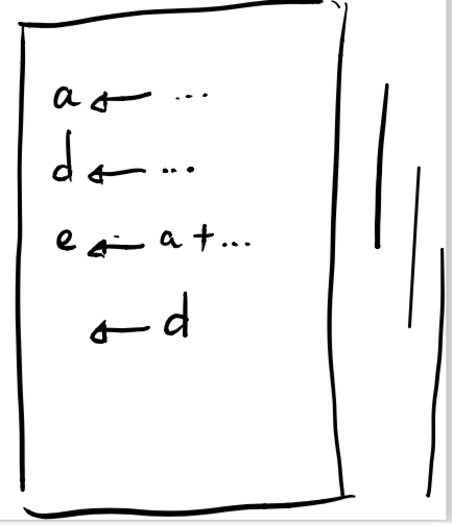
\includegraphics[width=0.27\textwidth]{figures/ra_linearscan.pdf}}
  \hfill
  \subfloat[Linear scan]{\usebox{\linearscanbox}}
    \caption{\label{fig:ra:linearscan}Linear scan assignment scheme on a basic-block: assigning registers to live intervals from top to bottom ($a$, then $d$, followed by $e$) always succeeds if \maxlive (here two) does not exceed the number of available registers. }
\end{figure}



That important observation gave rise to the linear scan register allocation scheme widely adopted by just-in-time compilers, as the algorithm is very fast.
However, for a general control-flow graph, the algorithm is not optimal, so classical register allocation schemes like to think of interferences as an undirected \emph{interference graph}: the nodes are the variables of the program, and two nodes are connected if they interfere.
A \emph{coloring} of this graph with~$k$ colors corresponds to a valid register allocation with~$k$ registers.\footnote{Hence the terms ``register'' and ``color'' will be used interchangeably in this chapter.}
A $k$-coloring is a mapping from the nodes of the graph to the first~$k$ natural numbers (called colors) such that two neighbouring nodes have different colors.
Unfortunately, graph $k$-coloring is known to be an NP-complete problem, and for any arbitrary undirected graph, there is a program whose interference graph is this graph.
This is the major nuisance of classical register allocation:
the compiler cannot efficiently determine if spilling is necessary,
which means one might need more registers than \maxlive.

The somewhat non intuitive result is that, even if at every program point there are no more than \maxlive variables alive, we still might need more than $\maxlive$ registers for a spill-free register allocation!
The causes of this problem are control-flow merges, as can be seen in Figure~\ref{fig:ra:exprg}.
In that example, the register pressure is at most two at every program point.
However, because the variable $e$ is defined in both branches of an if-condition, the interference graph cannot be colored with two colors: its \emph{chromatic number} is three.
The inequality between \maxlive and the chromatic number is caused by the cycle in the interference graph.


\begin{figure}[htbp]
	\begin{center}
		\subfloat[Example program and live-ranges of its variables]{ 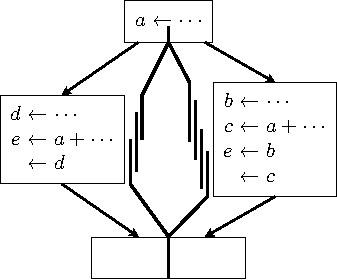
\includegraphics{figures/prog_lr.pdf}
                \label{sub:ra:exprg:prog}
                }
		\qquad
		\subfloat[Interference graph]{ 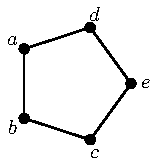
\includegraphics[scale=1.1]{figures/prog_ig.pdf} }
	\end{center}
	\caption{Example program and its interference graph}
	\label{fig:ra:exprg}
\end{figure}


This situation changes if we permit \emph{live-range splitting.} 
That is, inserting a copy (move) instruction at a program point that creates a new variable. 
Thus, the value of a variable is allowed to reside in different registers at different times. 
In Figure~\ref{sub:ra:exprg:prog}, assume we split the live-range of~$e$ in the left block: 
we rename it by~$e'$ and add a copy~$e \gets e'$ at the end of the block. 
Then, the node~$e$ in the graph is split into two nodes, $e$ and~$e'$, that do not interfere: 
this breaks the cycle in the graph, making its chromatic number equal to two, i.e., \maxlive. 
In an extreme setting, one could split the live-ranges of all variables after every instruction. 
The interference graph degenerates into several disconnected components and its chromatic number drops to \maxlive. 
Of course, such an extreme live-range splitting introduces \emph{a lot of shuffle code}, in the form of register to register copies, which degrades the run-time of the compiled program. 
This interplay between live-range splitting and colorability is the key issue in register allocation, and we will see in the remainder of this chapter how SSA, which creates live-range splitting at particular locations, can play a role in register allocation.
% (cf.~the SSA version of the program shown in Figure~\ref{fig:ra:exprgssa}). 

\begin{figure}[htbp]
	\begin{center}
		\subfloat[Example program with live-range of~$e$ split]{ 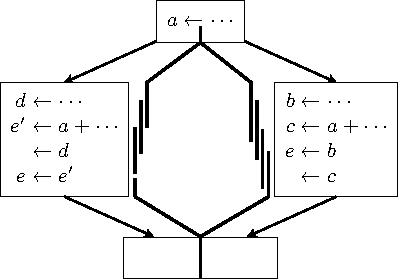
\includegraphics{figures/prog_split_lr.pdf} }
		\qquad
		\subfloat[Interference graph]{ 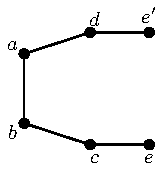
\includegraphics[scale=1.1]{figures/prog_split_ig.pdf} }
	\end{center}
	\caption{Example Program with spit live-range and its interference graph}
	\label{fig:ra:exprgsplit}
\end{figure}


\subsection{Making the spill test efficient: splitting or not splitting}
As finding a valid $k$-coloring is NP-complete, assigning registers is performed in classical register allocators by some heuristic algorithm.
If that algorithm fails to assign a register to a variable, then it either spills this variable to memory, or frees a register by spilling the variable it contains.
The problem here is that the spilling decision is made to revive the coloring heuristic, and not because the variable that gets spilled is in itself a good candidate for spilling. 
Even worse, we might spill a variable because the heuristic is ``not good enough,'' and not because we are actually out of registers!

In that regard, whatever the coloring heuristic, live-range splitting (up to the extreme setting of splitting at every program point) will never produce ``over-spilling'' decisions.
But if one wants to avoid spill code (memory loads and stores) as much as possible, too many register-to-register copies should also be avoided.
For that purpose, at the same time coloring and spilling decisions are made, classical algorithms also perform copy coalescing (i.e.,~undoing live-range splitting).
However, if done aggressively, coalescing may increase the chromatic number of the graph, or make the graph harder to color for the heuristic.
Thus, existing techniques often apply \emph{conservative} coalescing approaches which are guaranteed not to increase the chromatic number of the graph, at the expense of the quality of the coalescing.
The main issue with conservative coalescing is that, with an extreme solution that would split all live-ranges at every basic-block boundaries, it is either slow or inefficient in removing most of the spurious introduced copies.
Thus, the splitting or not splitting trade-off has to be addressed by the register allocator.
We will see that live-range splitting based on SSA form is an elegant solution to this trade-off problem as it is sufficient in bringing the interference graph \maxlive-colorable without blowing-up the number of live-ranges.

As already mentioned in Section~\ref{sec:properties_and_flavours:domprop} of Chapter~\ref{chapter:properties_and_flavors}, the live-ranges in an SSA form program with dominance property have interesting structural properties:
In that flavor, SSA requires that all uses of a variable are dominated by its definition.
Hence, the whole live-range is dominated by the definition of the variable.
Dominance, however, induces a tree on the control-flow graph.
Thus, the live-ranges of SSA variables are all tree-shaped.
They can branch downwards on the dominance tree but have a single root:
the program point where the variable is defined.
Hence a situation like in Figure~\ref{fig:ra:exprg} can no longer occur:
$e$~had two ``roots'' because it was defined twice.
Under SSA form, the live-range of~$e$ is split by a \phifun.
The argument and result variables of that \phifun constitute new live-ranges, giving more freedom to the register allocator since they can be assigned to different registers.

\begin{figure}[htbp]
	\begin{center}
		\subfloat[example program in SSA]{ 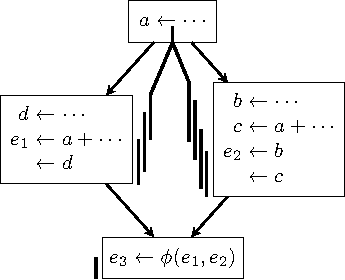
\includegraphics{figures/prog_ssa_lr.pdf} }
		\qquad
		\subfloat[Interference graph]{ 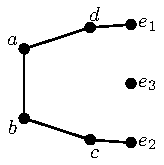
\includegraphics[scale=1.1]{figures/prog_ssa_ig.pdf} }
	\end{center}
	\caption{SSA version of the example program}
	\label{fig:ra:exprgssa}
\end{figure}

This structural property is interesting as it allows a coloring scheme, called the tree scan, that is a simple generalization of the linear scan mentioned above: 
it always succeeds in coloring the tree-shaped live-ranges with \maxlive colors. 
This greedy assignment scans the dominance tree, coloring the variables from the root to the leaves in a top-down order. 
This means the variables are simply colored in the order of their definitions, first come first served! 
We give the pseudo-code in procedure Tree\_Scan, Figure~\ref{code:assign-tree-scan}.
Intuitively, when the scanning arrives at the definition of a variable, the only colored variables are ``above'' it and since there is at most $\maxlive-1$ other variables live at the definition, there is always a free color. 
The direct consequence is that, as opposed to general form programs, the only case where spilling is required is when $\maxlive > k$. 
This allows to decouples spilling from coloring: 
First, lower the register pressure to~$k$ everywhere in the program; 
Then, color the interference graph with~$k$ colors in polynomial time.


\begin{figure}
  \begin{verbatim}
Tree_Scan(T)
  function assign_color(p, available)
    for each v last use at p
      available[color(v)] = True     /* colors not used anymore */
    for each v defined at p
      c = choose_color(v, available)  /* choose available color */
      available[c] = False
      color(v) = c
    for each child p' of p
      assign_color(p', available)
  assign_color(root(T), [True, True, ..., True])

  \end{verbatim}
  \caption{Tree scan coloring algorithm for SSA.}
  \label{code:assign-tree-scan}
\end{figure}


\section{Spilling}

The term spilling is heavily overloaded:
In the graph-coloring setting it often means to spill a node of the interference graph and thus the \emph{entire} live-range of a variable (spill everywhere).
This implies inserting load instructions in front of every use and store instructions after each definition of the (non-SSA) variables.
In practice, a post-pass of a graph coloring scheme scans each basic-block separately, so as to, whenever possible, keep a reloaded variable in a register between multiple uses (an optimization also used in linear scan allocators).
In this section, we will consider the two approaches: the graph-based approach with a spill-everywhere scheme, and scan-based approach that allows partial live-range spilling.

In both cases, we will assume that the program was in SSA before spilling. 
This is important to notice that there are pros and cons of assuming so. 
In particular, the inability to coalesce or move the shuffle code associated to \phifuns can lead to spurious load and store instructions on CFG-edges. 
However, we do make the exercise of considering this assumption here, and consider the spilling phase as an SSA program transformation.
Suppose we have $R$ registers, its objective is to establish $\maxlive\le\regs$ (\maxlive lowering) by inserting loads and stores into the program. 
Indeed, as stated above, lowering \maxlive to~\regs ensures that a register allocation with \regs registers can be found in polynomial time for SSA programs. 
Thus, spilling should take place before registers are assigned \emph{and} yield a program in SSA form. 
In such a decoupled register-allocation scheme, the spilling phase is an optimization problem for which: 
\begin{itemize}
  \item the \emph{constraints} that describe the universe of possible solutions expresses that the resulting code should be \regs-colorable; 
  \item the \emph{objective function} expresses the fact that the (weighted) amount of inserted loads and stores should be minimized.
\end{itemize}

In a greedy scheme, the constraints give rise to the ``spill test'' which can be expressed as: 
is more spilling necessary or not? 
The objective is expressed with the profitability test: 
among all variables, which one is more profitable to spill? 
The main implication of spilling in SSA programs is that the spill test---which amounts to checking whether \maxlive has been lowered to \regs or not---becomes precise. 

The other (related) implication of the use of SSA form follows from this observation: 
Consider a variable such that for any program point in its entire live-range the register pressure is lower than \regs, then spilling this variable is useless with regard to the colorability of the code.
In other words, spilling such a variable will never be profitable. 
We will call this yes-or-no criteria, enabled by the use of SSA form, the ``usefulness test.''
Among all useful-to-spill variables, the question is whether the use of SSA form allow to improve the quality of the profitability test.
While there are no experimental results that allow to assess the correctness of this assertion, it seems that the enabled capability to decouple spilling  (allocation) to coloring (assignment) allows to better account for the program structure in the spilling decision, and thus improve the overall quality of register allocated code.
After a brief description of how the usefulness test can be implemented in a graph coloring based scheme, the goal of the next section is to argue in favor of a scan based scheme for spilling decision.

\subsection{Graph-based approach}

FLO: TODO : parler d'IRC.

We need to find program points to place loads and stores such that $\maxlive\le\regs$.
Let us start with a simplistic setting where the location of loads and stores is not optimized:
loads are placed directly in front of uses and stores directly after the definition.
Most existing graph coloring schemes consider a \emph{spill everywhere} setting:
a variable is either spilled completely or not at all;
If spilled, the live-range of a variable then degenerates into small intervals: one from the definition and the store, and one from each load to its subsequent use.
However, even in this simplistic setting, it is NP-complete to find the minimum number of nodes to establish $\maxlive\le\regs$.
It is even NP-complete to find the minimum number of nodes to spill to decrease \maxlive just by one!
Existing graph coloring schemes greedily spill variables (graph nodes) using a weight that usually combines its node degree (number of interfering uncolored variables) and an estimated spill cost (estimated execution frequency of inserted loads and stores).
The node degree amounts to evaluate the profitability of spilling the node in terms of colorability.
This criteria can be enhanced by adding a usefulness tag as follow:

The interference graph is built through a simple traversal of the CFG: 
To an interference-graph node $p$ is associated an SSA program variable $p.\textit{var}$ and vis-versa. 
There is an interference edge $(v,p)$ from $v$ to $p$ if and only if $v.\textit{var}$ is alive at $p.\textit{var}$ definition point. 
Observe that, as opposed to standard interference graphs, we consider directed edges here. 
Also, to each node $p$, we associate a field $p.\textit{pressure}$ that corresponds to the number of variable alive at definition point of $p.\textit{var}$. 
As the edge $(v,p)$ is added to the graph, a boolean $(v,p).\textit{high}$ is set with value \true if and only if $p.\textit{pressure}>\regs$. 
Another field $v.\textit{useful}$, that is attached to every node $v$ is also updated: 
if $p.\textit{pressure}>\regs$ then $p.\textit{useful}$ is set to 1 (otherwise set to 0), and for all $(v,p)$, $p.\textit{pressure}$ gets incremented by 1 (other nothing is done). 
At the end of the build process, $v.\textit{useful}$ expresses the number of program points that belong to the live-range of $v.\textit{var}$ and for which the register pressure is greater than \regs. 
In other words,
$$v.\textit{useful}=\left|\lbrace p,\ p.\textit{pressure}>\regs \wedge\left(\exists (v,p) \vee v=p \right) \rbrace\right|$$
Defined as it, if $v.\textit{useful}=0$, then it can be considered to be be useless to spill $v$.
If not, it means that $v$ belongs to a clique of size greater than $\regs$, and that one of the nodes of the clique must be spilled. 
In that case, spilling $v$ is useful as it would reduce the size of the clique by one.

Whenever a node $n$ is spilled (assume only useful nodes are spilled), those additional fields of the interference graph are updated as follow:
1.~if $n.\textit{pressure}>\regs$, for all its incoming edges $(v,n)$, $v.\textit{useful}$ is decremented by one;
2.~for all its high outgoing edges $(n,p)$, $p.\textit{pressure}$ is decremented by one; if following this decrement $p.\textit{pressure}$ becomes equal to \regs, then for all the incoming edges of $p$ $(v,p)$, $v.\textit{useful}$ is decremented by one.

As one can observe, as spilling and coloring decisions are fully decoupled now, encoding the information using a graph does not seem to help much. 
Moreover, formulations like \emph{spill everywhere} are often not appropriate for practical purposes, and putting the whole live-range to memory is too simplistic. 
A variable might be spilled because at some program point the pressure is too high; 
However, if that same variable is later used in a loop where the register pressure is low, a spill everywhere will place a superfluous (and costly!) load in that loop. 
Spill everywhere approaches try to minimize this behavior by adding costs to variables, to make the spilling of such a variable less likely. 
These bring in a flow-insensitive information that a variable reside an frequently executed area. 
However, such approximations are often too coarse to give good performance. 
Hence, it is imperative to cleverly split the live-range of the variable according to the \emph{program structure} and spill only parts of it.


\subsection{Scan-based approach}
In the context of a basic block, a simple algorithm that works well is the ``furthest first'' algorithm (see Figure~\ref{fig:ra:ff}). 
The idea is to scan the block from top to bottom.
Whenever the register pressure is too high, the spilled variable is the one whose next use is the furthest away (expressed as maximizing \verb+distance_to_next_use_after(p)+ in function \verb+evict+ of Figure~\ref{fig:ra:ff}); 
And it is spilled only \emph{up to this next use}. 
Spilling this variable frees a register for the longest time, hence diminishing the chances to have to spill other variables later. 
This algorithm is not optimal since the first time a variable is spilled, a load and a store are added; 
For subsequent spilling of the same variable (but on a different part of its live-range), only a load must be added. 
Hence this algorithm may produce more stores than necessary (e.g., by spilling two variables while spilling an other part of the first one would have been enough), but it gives good results on ``straight-line code,'' i.e., basic blocks.

\begin{figure}
\begin{verbatim}
Further_First(B)
  function evict(p, &in_regs, &in_mem, in_solidstate)
    while |in_regs|>R
      let v in (in_regs - in_solidstate) with max v.distance_to_next_use_after(p)
      if v not in in_mem 
         insert a store of v to memory just before p
         in_mem = in_mem U {v}
      in_regs = in_regs \ {v}

  foreach prog point p in B from top to bottom
    #uses of v must be in a register before p
    foreach v used at p
       if v not in var_in_regs 
          insert a load of v from memory just before p
          var_in_regs = var_in_regs U {v}
    evict(p, var_in_regs, var_in_mem, var_to_load)
    #there must be space for vars defined at p
    foreach v last use at p  
      var_in_regs = var_in_regs \ {v}
    foreach v defined at p
      var_in_regs = var_in_regs U {v}
    evict(p, var_in_regs, var_in_mem, {vars defined at p})
\end{verbatim}
\caption{\label{fig:ra:ff}Further First spilling algorithm for straight-line code}
\end{figure}

We now present an algorithm that extends this ``furthest first'' algorithm to general control-flow graphs.
The idea is to scan the CFG using a topological order and greedily evict sub live-ranges whenever the register pressure is too high.
There are two main issues:
the first is to generalize the priority function \verb+distance_to_next_use_after+ to a general CFG;
the second is to find a way to initialize the \verb+in_regs+ set when starting to scan a basic-block, in the situation where predecessor basic-blocks have not been processed yet (e.g. at the entry of a loop).

\paragraph{Profitability to Spill}
To illustrate the generalization of further-first priority strategy to a CFG, let us consider the example of Figure~\ref{fig:ra=priority-spill-CFG}.
In this figure, $\lightning n$ sign denotes regions with (high) register pressure of $\regs+n$.
Here, at program point $p_0$, register pressure is too high by one variable:
both $x$ and $y$ are candidate to be spilled to memory.
\begin{enumerate}
\item Let us first consider the execution trace ($AB^{100}C$) under the assumption that left branch is taken. 
  In this branch, next use of $y$ appears in a loop, while next use of $x$ appears way further once the loop have fully executed. 
  Looking at this execution trace in isolation, and using the further first strategy described above for straight-line code, it is clearly considered to be more profitable to evict variable $x$ (at distance 101).
\item Consider now the execution trace ($AD$) whenever the right branch is taken. In that case, this is variable $y$ has the further use (at distance 2).
\item Looking at the example as a whole, it is clear that one would prefer to evict variable $y$. 
  On the other hand, modifying a little bit the example by assuming a high register pressure within the loop at program point $p_1$, then evicting variable $x$ would be preferred.
\end{enumerate}
This dictates the following remarks:
First, program points with low register pressure can be ignored.
Second, program points within loops, or more generally said with higher execution frequency should account in the computation of the ``distance'' more than program points with lower execution frequency.
%
This leads, for a variable $v$ live at program point $p$ to the following definition of function \verb+v.spill_profitability(p)+ where $q.\texttt{frequency}$ represents the estimated execution frequency for a program point $q$:

\begin{figure}
  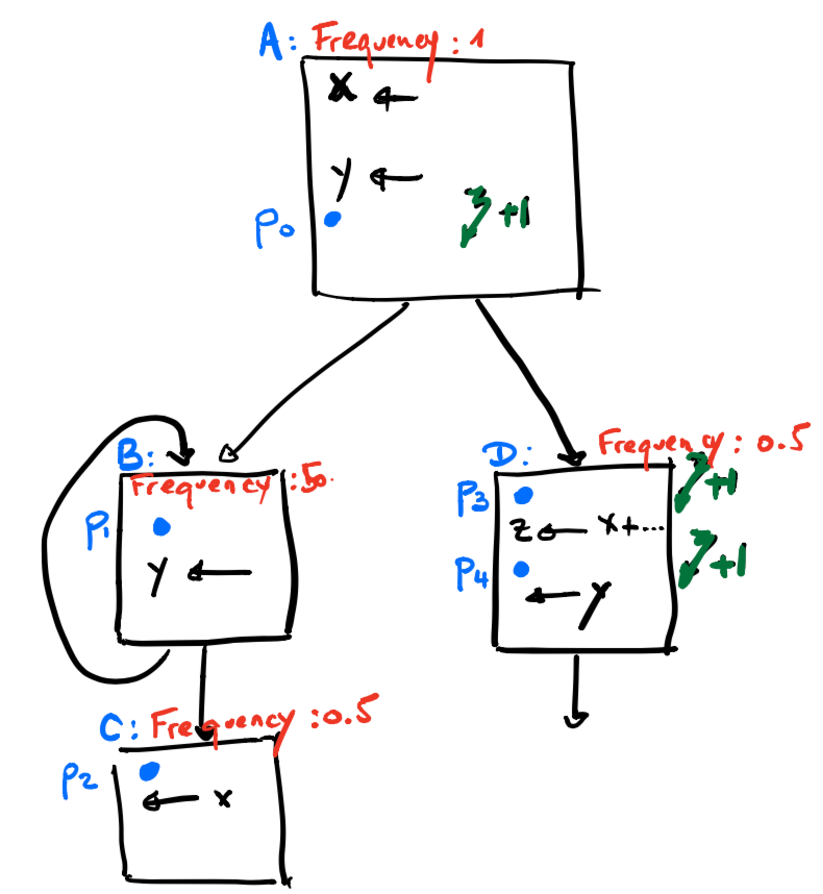
\includegraphics[width=0.45\textwidth]{figures/priority-spill-CFG.pdf}
  \caption{\label{fig:ra:priority-spill-CFG}Generalization of \texttt{distance\_to\_next\_use\_after} for a CFG. Illustrating example.}
\end{figure}

\begin{definition}[Spill profitability from $p$]
  Let $p$ be a program point, $v$ a variable live at $p$.
  Let $v.\texttt{HP}(p)$ be the set of all program points $q$ such that:
  1.~register pressure at $q$ is greater than \regs;
  2.~$v$ is alive at $q$;
  3.~there exists a path from $p$ to $q$ that does not contain any use or definition of $v$.
  Then,
  $$\texttt{v.spill\_profitability}(p) = \sum_{q\in v.\texttt{HP}(p)} q.\texttt{frequency}$$
\end{definition}

There is a important subtlety concerning the set of points in $v.\texttt{HP}(p)$, that is aimed to express the set of program points of high register pressure for which the eviction of $v$ would free a register:
depending on the instruction set architecture, and the way spill code is inserted, it might be desirable to consider the use point of an instruction, just before the instruction itself (where the load would have been to be inserted).
This, for example, would lead as illustrated below in our running example, to exclude $p_3$ from $x.\texttt{HP}(p_0)$.
Hence,
\begin{enumerate}
\item assuming low register pressure within the loop, we have $x.\texttt{HP}(p_0)=\{p_0\}$, and $y.\texttt{HP}(p_0)=\{p_0,p_3\}$. 
  This leads to $x.\texttt{spill\_profitability}(p_0)=1$ and $y.\texttt{spill\_profitability}(p_0)=1+0.5=1.5$, ie. evicting $y$.
\item now assume register pressure to be high at $p_1$, then $x.\texttt{HP}(p_0)=\{p_0,p_1\}$, and $y.\texttt{HP}(p_0)=\{p_0,p_3\}$. This leads to $x.\texttt{spill\_profitability}(p_0)=1+50=51$ and $y.\texttt{spill\_profitability}(p_0)=1.5$, i.e. evicting $x$.
\end{enumerate}

\paragraph{Initial Register Filling at the Beginning of a Basic-Block}
For each visited basic-block $B$, the set of variables that must reside in a register is stored in \verb+B.vars_in_regs+.
For each basic-block, initial value of this set has to be computed prior to starting processing it.
The heuristic for computing this set is different for a ``normal'' basic-block and for a loop entry.
For a normal basic-block, as we assume a topological order traversal of the CFG, all its predecessors have been processed yet.
Live-in variables fall into three sets:
\begin{enumerate}
\item the ones that are available in all predecessor basic-blocks:
  $$B.\texttt{allpreds\_in\_regs}=\bigcap_{P\in \textrm{pred}(B)} P.\texttt{in\_regs}$$
\item the ones that are available in some of the predecessor basic-blocks:
  $$B.\texttt{somepreds\_in\_regs}=\bigcup_{P\in \textrm{pred}(B)} P.\texttt{in\_regs}$$
\item the ones that are available in none of them.
\end{enumerate}
As detailed in Figure~\ref{fig:ra:initnormal}, $B.\texttt{in\_regs}$ is initialized with $B.\texttt{allpreds\_in\_regs}$ plus, as space allows, elements of $B.\texttt{somepreds\_in\_regs}$ sorted in decreasing order of their \texttt{spill\_profitability} metric.

\begin{figure}
\begin{verbatim}
Init_inregs(B)
  allpreds_in_regs = Union for all P in B.preds of P.in_regs
  somepreds_in_regs = Intersection for all P in B.preds of P.in_regs
  B.in_regs = allpreds_in_regs
  while |B.in_regs| < R and |somepreds| > |B.in_regs|
    let v in (somepreds - B.in_regs) with min v.spill_profitability(B.entry)
    B.in_regs = B.in_regs U {v}
\end{verbatim}
\caption{\label{fig:ra:initnormal}Initial value of $B.\texttt{in\_regs}$ for normal basic-block}
\end{figure}

\begin{figure}
  \begin{center}
    \subfloat[\label{fig:ra:loopentry_example_a}\texttt{in\_regs} at $B$'s entry]{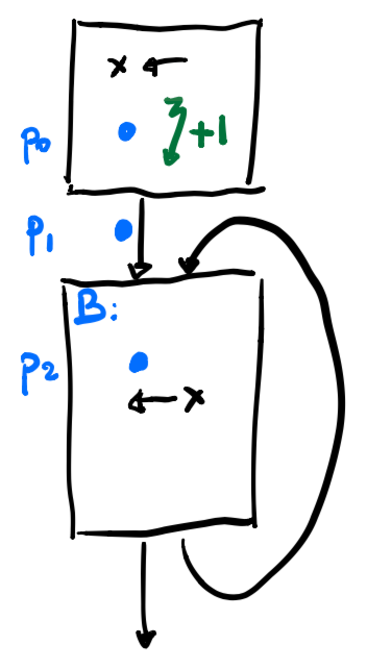
\includegraphics[width=0.15\textwidth]{figures/loopentry_example_a.pdf}}
    \qquad
    \subfloat[\label{fig:ra:loopentry_example_b}not \texttt{in\_regs} at $B$'s entry]{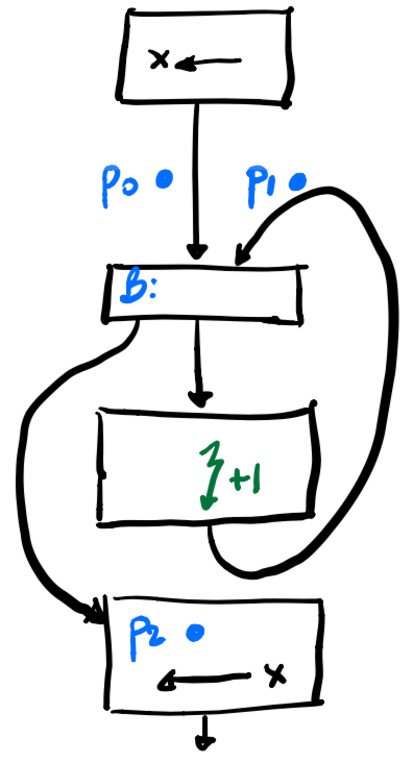
\includegraphics[width=0.15\textwidth]{figures/loopentry_example_b.pdf}}
  \end{center}
  \caption{\label{fig:ra:loopentry_example}Initial values of $B.\texttt{in\_regs}$ at loop entry. Illustrating examples.}
\end{figure}
For a basic-block at the entry of a loop, as illustrated by the example of Figure~\ref{fig:ra:loopentry_example}, one do not want to account for allocation on predecessor basic-block, but start from scratch instead.
Assume the first basic-block has already been processed and one wants to compute $B.\texttt{in\_regs}$:
\begin{enumerate}
\item Take Example~(a): 
  Even if at the end of the predecessor basic-block , $x$ is not available in a register, one wants to insert a reload of $x$ at $p_1$, i.e. include $x$ in $B.\texttt{in\_regs}$.
  Not doing so would involve a reload at every iteration of the loop at $p_2$. 
\item Consider Example~(b): 
  Even if at the entry of the loop, $x$ is available in a register, one wants to spill it and restore at $p_2$ so as to lower the register pressure that is too high within the loop.
  This means excluding $x$ from $B.\texttt{in\_regs}$.
\end{enumerate}
This leads to the algorithm given in Figure~\ref{fig:ra:initloop} where $B.\texttt{livein}$ represent the set of live-in variables of $B$ and $L.\texttt{MAXLIVE}$ is the maximal register pressure in the whole loop $L$.
\texttt{Init\_inregs} first fills $B.\texttt{in\_regs}$ with live-in variables that are used within the loop $L$.
It then, fills with live-through variables, but only those that can survive the loop:
if $L.\texttt{MAXLIVE}>\regs$, then  $L.\texttt{MAXLIVE}-\regs$ variables will have to be spilled (hopefully some live-through variables);
so no more than $|B.\texttt{livein}|-(L.\texttt{MAXLIVE}-\regs)$ are allocated to a register at the entry of $B$.

\begin{figure}
\begin{verbatim}
Init_inregs(B,L)
  B.in_regs = emptyset
  while |B.in_regs| < R  and
        |B.livein| > |B.in_regs| and
        |B.in_regs| < R + |B.livein| - L.MAXLIVE
    let v in (B.livein - B.in_regs) with min v.spill_profitability(B.entry)
    B.in_regs = B.in_regs U {v}
\end{verbatim}
\caption{\label{fig:ra:initloop}Initial value of $B.\texttt{in\_regs}$ at the entry of a loop $L$}
\end{figure}

\paragraph{Putting all Together}
The overall algorithm for spilling is made-up of several phases:
First, both liveness, and profitability metric have to be pre-computed.
Then the traversal in topological order of the CFG can be done, where each basic-block is scanned using initial value of \verb+B.in_regs+ as explained above.
During this phase, the sets of live-variables respectively available in register and in memory are maintained at basic-block boundaries.
This allows the insertion of shuffle code (loads and store) performed during the last phase of the algorithm.

\section{Coloring and coalescing}

In a decoupled register allocation scheme as advocated here, the spilling phase first lowers the register pressure so that $\maxlive \leq \regs$.
With the help of live-range splitting through the insertion of register-to-register copies, then no more than \regs registers are required to successfully allocate variables.
Now, SSA form has the good property that it provides sufficient live-range splitting.
Also, when dressed with its minimal flavor (see Chapter~\ref{cahpter:properties_and_flavors}), the increase in terms of variables is reasonable (usually less than 20 percent in practice) compared to splitting all global live-range at the border of every basic-block.
The fact that a greedy tree-scan coloring scheme (see Figure~\ref{code:assign-tree-scan}) can ``optimally'' do the job, is quite useful property of SSA form.
Even more interestingly, one of the goal of this section is to show that the underlying structural property is such that it also makes the extensively used graph coloring simplification scheme (recalled below) an ``optimal'' scheme.
In other words, the well-known iterated register allocation scheme can take advantage of SSA form property.
This is especially important remark because, besides minimizing the amount of spill code, the second objective of register allocation is to also minimize the amount of register-to-register copies:
a decoupled approach is practically viable if the coalescing phase is effective in merging most of the live-ranges.
In this section, we will first present the traditional simplification scheme based graph coloring greedy heuristic and show how it successfully color programs under SSA form.
We will then explain how those two greedy coloring schemes, respectively the graph-based and the scan-based (described in Figure~\ref{code:assign-tree-scan}), can be extended to perform efficient coalescing.

 

\subsection{Greedy coloring scheme}
\label{sec:ra:greedy-col}

In traditional graph coloring register allocation algorithms, the assignment of registers to variables is done by coloring the interference graph using a greedy heuristic.
This scheme is based on the observation that given \regs colors---representing the registers---, if a node in the graph has at most $\regs-1$ neighbors, there will always be one color available for this node whatever colors the remaining nodes have.
Such a node can be \emph{simplified}, i.e., removed from the graph and placed on a stack.
This process can be iterated with the remaining nodes, whose degree may have decreased (if the simplified node was one of their neighbors).
If the graph becomes empty, we know it is possible to color the graph with \regs colors; 
In particular, as illustrated in Figure~\ref{code:assign-color}, a valid \regs-coloring can be obtained by assigning colors to nodes in the reverse order of their simplification, i.e., popping nodes from the stack and assigning them one available color.
This is always possible since they have at most $\regs-1$ colored neighbors.
We call this algorithm the \emph{greedy coloring scheme}.\index{greedy coloring scheme}
Its first phase, which goal is to eliminate nodes from the graph to create the stacks is reported in Figure~\ref{code:is-k-greedy}.


\begin{figure}
\begin{verbatim}
Function Simplify(G)
  Data: Undirected graph G = (V, E);
  For all v, degree[v] = #neighbours of v in G,
  k number of colors
stack = {} ;
worklist = {v in V | degree[v] < k} ;
while worklist != {} do
  let v in worklist ;
  foreach w neighbour of v do
    degree[w] = degree[w]-1 ;
    if degree[w] = k - 1 then worklist = worklist U {w}
  push v on stack ;
  worklist = worklist \ {v} ; /* Remove v from G */
if V != {} then Failure ``The graph is not simplifiable''
return stack ;
\end{verbatim}
\caption{Iskgreedy function}
\label{code:is-k-greedy}
\end{figure}


The greedy scheme is a coloring heuristic, and as such, it can get stuck;
it happens whenever all remaining nodes have degree at least \regs.
In that case, we do not know whether the graph is \regs-colorable or not.
In traditional register allocation, this is the trigger for spilling some variables so as to unstuck the simplification process.
However, as explained below, under the SSA form, if spilling has already been done so that the maximum register pressure is at most \regs, the greedy coloring scheme can never get stuck!
Consider the greedy simplification scheme described above, and picture the dominance-tree with live-ranges as sub-trees of this tree.
At the end of each dangling branch there is a ``leaf'' variable, that is defined last in this branch.
We can visually see that this variable will not have many intersecting variables:
those are the variables alive at its definition point, i.e. no more than \regs-1 (\maxlive being lower than \regs).
It is in fact a candidate for simplification, and once removed another variable will become the new leaf.
We see that simplification can always happens at the end of the branches of the dominance tree, moving upwards until the whole tree is simplified.
In other words, if we are under SSA form and the spilling has already been done so that $\maxlive \leq R$, the classical greedy coloring scheme is \emph{guaranteed} to perform register allocation with \regs colors without any additional spilling.
Observe that, with a program originally under SSA form, practical implementation may chose to interleave the process of spilling and coalescing/coloring:
result will be unchanged but speed might be impacted.
This is practical for instance when working on an existing compiler that uses a classical register allocation algorithm, for instance, the Iterated Register Coalescing.



\begin{figure}
\begin{verbatim}
Function Assign_colors(G)
  available = new array of size R and values True
  while stack != {} do
    v = pop stack ;
    for each neighbor w in G
      available[color(w)] = False
    col = 0;
    for each color c from 1 to R
      if available[c]
        col = c
      available[c] = True /* prepare for next round */
    color(v) = col
    add v to G
\end{verbatim}
\caption{Assign\_color function}
\label{code:assign-color}
\end{figure}


FAB: JE SUIS ICI MAIS JE VAIS RELIRE LE TRUC DESSUS AVANT DE CONTINUER
\subsection{A light tree-scan coloring algorithm}
{\sl
\begin{itemize}
  \item On the dominance tree, possible to scan from top and assign colors to 
    variables as they come.
  \item Biased coloring is used to coalesce variables linked by \phifuns.
  \item see next section for more involved coalescing
  \item Fab: I think that you already talked about scan coloring. Ok to talk about biased.
  \item Fab: You can talk about biased coloring that uses the result of an aggressive coalescing (see with Quentin). It is not more complicated and it improves results.
\end{itemize}
}

One of the advantages of SSA is to make things simpler, faster, and use less memory. 
For the register assignment problem, we now know that the existing greedy scheme based on simplification still works; 
However, it requires constructing and maintaining the interference graph, a structure judged to big and cumbersome to be used in a JIT context, where compilation time and memory prints matter more. 
We will now show how to perform a fast register assignment for SSA after spilling that does not need more than the dominance tree and def-use chains. 

%% The algorithm we propose scans the dominance tree, coloring the variables from the root to the leaves in a top-down order.
%% This means the variables are simply colored in the order of their definitions, first come first served!
%% We give the pseudo-code in procedure Tree\_Scan, Figure~\ref{code:assign-tree-scan}; It works because it mimics the effect of the greedy scheme (``leaves'' are simplified first hence colored \emph{last}), without actually performing any simplification.

%% Intuitively, when the scanning arrives at the definition of a variable, the only colored variables are ``above'' it and since there is at most $R-1$ other variables live at the definition, there is always a free color.
%% We will now prove more formally that this method always work;
%% The key observation is that the order in which variables are considered corresponds to a reverse order of simplification, i.e., a valid order of the nodes on the stack after the greedy simplification scheme.

%% \begin{proof}
%%   \def\order{o}
%%   Let us consider an ordering $v_1, v_2, \ldots, v_n$ of the nodes of the nodes based on the dominance:
%%   if $v_i$ dominates $v_j$, then $v_j$ appear before $v_i$ in the ordering ($j < i$).
%%   We will show that this order correspond to a greedy simplification.
%%   Suppose $v_1, \ldots, v_{i-1}$ have been simplified by the greedy scheme (for $i=1$, this is the initial graph).
%%   If $v_i$ dominates any variable, say $v_j$, then $j < i$ and the node has already been simplified;
%%   So, there is no variable defined after $v_i$ on the dominance tree:
%%   the live-range of $v_i$ is a ``leaf'' of the subtree representation (see proof in Section~\ref{sec:regalloc:ssa-greedy}).
%%   So, $v_i$ can be chosen for simplification, and by induction the ordering $v_1, \ldots, v_n$ is a valid order of simplification. 
%%   As we have seen previously in Section~\ref{sec:regalloc:greedy-col}, this means the reverse order $v_n, v_{n-1}, \ldots, v_1$ is a valid order for coloring.
%% \end{proof}


%% \begin{important}
%% It is important to understand why this method does not work in the general non-SSA case.
%% Under SSA, the variables are ``split'' at join points by the use of \phifuns.
%% If this was not the case, we would have live-ranges that spans on multiple branches of the dominance tree, creating cycles in the representation.
%% In that case, coloring a branch would constrain the coloring on leaves on a different branch; Under SSA form, such live-ranges are split and their colorings are independent.
%% See Figure~\ref{TODO} for an example.
%% \end{important}




The tree-scan coloring algorithm is really fast as it only needs one traversal of the dominance tree. 
Since the number of colors is fixed and small, it can be implemented as a bit-set to speed-up updates of the {\tt available} array.
The pseudo-code for function {\tt choose\_color} is deliberately not given yet. 
A very basic implementation could just scan the {\tt available} array until it finds one that is not taken.
We will see in the next section how to bias the choosing of colors so as to perform some coalescing. 
 


\subsection{Coalescing under SSA form}

The goal of \emph{coalescing} is to minimize the number of register-to-register {\tt move} instructions in the final code.
While there may not be so many such ``copies'' at the high-level (e.g., instruction ``{\tt a = b;}'' in C)---especially after a phase of copy propagation under SSA (\todo{See chapter X})---,
many such instructions are added by different compiler phases by the time compilation reaches the register allocation phase.
For instance, adding copies is a common way to deal with register constraints (see Section~\ref{sec:practical-regalloc}). 
An even more obvious and unavoidable reason in our case is the presence of \phifuns due to the SSA form. 

A \phifun represents in fact parallel copies on incoming edges of basic blocks. 
For instance, $a \gets \phi(b,c)$ means that instruction $a\gets b$ should be executed on the edge coming from the left, and $a\gets c$ on the one from the right. 
Suppose now that register allocation decided to put $a$ and $b$ in register $R_1$, but $c$ in register $R_2$;
Then, the copy $a\gets b$ does not need to be executed anymore, but $a\gets c$ still does:
the value of variable $c$ will be contained in $R_2$ and needs to transfered to $R_1$, which means the final code will contain an instruction ``{\tt mov $R_1, R_2$}'' or the like. 


In the case of SSA, it is obviously better to assign variables linked by a \phifun, to the same register, so as to remove copies between subscripts of the same variable ($a_1$, $a_2$, \dots).
This is possible if we are under conventional SSA (CSSA, see Chapter~\ref{todo}), but optimizations can break this property and interferences can appear between subscripted variables with the same origin.
Such two variables cannot be assigned to the same register without breaking the program.

To bypass this problem and also allow for more involved coalescing between SSA variables of different origins,
we define a notion of \emph{affinity}, acting as the converse of the relation of interference and expressing how much two variables ``want'' to share the same register. 
By adding a metric to this notion, it measures the benefit one could get if the two variables were assigned to the same register:
the weight represents how much instructions we would save at execution if the two variables share the same register.
For instance, given two variables $a$ and $b$, the weight of the affinity between them is the number of occurrence of copy instructions involving them ($a\gets b$ or $b\gets a$) or \phifuns ($a\gets\phi(\ldots,b,\ldots)$ or $b\gets\phi(\ldots,a,\ldots)$).
Actually, some parts of the program are more often executed than others, and a more accurate cost for each copy can be calculated using actual execution frequencies based on profiling;
It is also possible to use empirical parameters, for instance $\times 10$ for each level of nested loop, $\times 0.5$ if in a conditional branch, etc.


\subsubsection{Biased coalescing}

Since the number of affinities is sparse compared to the number of possible pairs of variables,
it is best to keep for each variable $v$ an ``affinity list'' where each element is a pair $(u,w)$ meaning that $v$ has an affinity with $u$ of weight $w$.
We propose a version of function {\tt choose\_color} that bias the choosing of colors based on these affinity lists, shown on Figure~\ref{code:choose-color}. 
The bias is very simple: each choice of color maximizes locally---under the current knowledge---the coalescing for the variable being colored. 
It is not of course optimal since the general problem of coalescing is NP-complete, and biased algorithms are known to be easily misguided. 


\begin{figure}
  \begin{verbatim}
global variables
  count = array of size #colors and containing only zeros

choose_color(v, available)
  for each (u,weight) in affinity_list(v)
    count[color(u)] += weight
  max_weight = -1
  col = 0
  for each color c
    if available[c] == true /* color is not used by a neighbour of v */
      if count[c] > max_weight
        col = c
        max_weight = count[c]
    count[c] = 0 /* prepare array for next call to choose_color */
  \end{verbatim}
  \caption{Choosing a color with a bias for coalescing.}
  \label{code:choose-color}
\end{figure}


\subsubsection{Aggressive coalescing to improve biased coalescing.}

There is another simple and interesting idea to improve biased coalescing. We 
still consider a JIT context where compilation speed is very important.
\todo{what kind of aggressive? Ask fab\ldots}


\subsubsection{More involved coalescing strategies}

It is beyond the scope of this book to describe in details deeply involved strategies for coalescing.
So we will just give a short overview of other coalescing schemes that might be use in a decoupled register allocator.
\begin{itemize}
  \item Iterated Register Coalescing: conservative coalescing that works on the interference graph
  \item Brute force strategy, working on all ``greedy-$k$-colorable'' graphs
\end{itemize}




\section{Practical and advanced discussions}
\label{sec:practical-regalloc}


\subsection{Handling registers constraints}

In theory, register allocation algorithms are always nicely working with nodes 
and colors. In practice, however, not all variables or registers are 
equivalent. Depending on the architecture, some registers might be dedicated 
to perform memory operations, some instructions expects their operands to 
reside in particular registers, and in general conventions are defined to 
simplify for example the writing of libraries, by specifying how parameters to 
functions are passed and how results are returned. This adds constraints to the 
register allocation, usually by restricting the coloring possibilities of 
variables. Some examples are given in Figure~\ref{fig:reg-constraints}.

\begin{figure}
  \begin{center}
    \begin{tabular}{llcc}
    Context & Constraint  & Instruction & Effect on reg. alloc. \\
    x86 & Division in registers $R_x$ and $R_y$ & $a / b$ & $a$ in $R_x$, $b$ in $R_y$\\
    st200 & Memory load cannot use $R_z$ & $a = load(b)$ & $b$ cannot be in $R_z$\\
    ABI & Functions arguments in $R_1$, $R_2$\ldots & $a = f(b,c)$ & $b$ in $R_1$, $c$ in $R_2$ \\
     & result in $R_0$ & & $a$ in $R_0$\\
  \end{tabular}
  \end{center}
  \caption{Examples of register constraints.}
  \label{fig:reg-constraints}
\end{figure}


The problem with such constraints is that they cannot be expressed directly in 
the register allocation problem under SSA form. For instance, if variable $a$ and $b$ must 
absolutely reside in register $R_1$, it is not possible to pre-color them with 
color $R_1$ as the interference graph could not be chordal anymore.  
Furthermore, $a$ and $b$ maybe interfere, for instance if they are both the 
first parameter of successive function calls. In that case putting them in the 
same register would break the program. We propose two solutions 
to deal with this problem. The first is classic in the literature, and the 
second is newer and promising.


\paragraph{Splitting variables to handle register constraints.}

Traditionally, variables involved in constraining operations are split before and after the operation.
For instance, suppose $a$ is involved in an instruction that requires it to be in register $R_x$.
Then the instructions $a'\gets a$ and $a\gets a'$ are issued before and after the division,
$a'$ is forced to be in $R_x$ and is used instead of $a$ in the instruction.
If $a$ happens to be in $R_x$ after the register allocation, the copies can be removed, if not, the copies ensure the constraint is respected.

In SSA form, the problem is that variable $a'$ is $R_x$, and if this constraint appears somewhere else in the program, it breaks the SSA property since there would be multiple definition of the same variable.
Additionally, $a$ also is redefined which also breaks the SSA form.

A workaround solution is to split \emph{all} variables alive before and 
after the operation using a \emph{parallel copy}, as shown on Figure~\ref{fig:reg-split-all}.
Moreover, the second copy must must define new variables to keep the SSA property (and subsequent uses must be changed accordingly).

The use of parallel copies assures that the locally created variables, with very short live-ranges (span of only one instruction), are completely disconnected from the rest of the interference graph.
Their only relation with the other, ``normal'' variable are affinities that each 
variable share with the two other parts coming from the same original variable.

The only problem with this method is that many copy instructions can remain in the program if the coalescing is not good enough to assign most of the created variables to the same register.  

\begin{figure}
  \begin{minipage}{.39\textwidth}
  \begin{center}
    Before
      \begin{verbatim}
Live in = {a, b, c, d, e}

f = a/b

Live out = {a, c, d, e, f}

      \end{verbatim}
  \end{center}
  \end{minipage}
  \begin{minipage}{.6\textwidth}
  \begin{center}
    After
      \begin{verbatim}
Live in = {a, b, c, d, e}

(a', b', c', d', e') = (a, b, c, d, e)

f' = a'/b'

(a'', c'', d'', e'', f) = (a', c', d', e', f')

Live out = {a'', c'', d'', e'', f}
      \end{verbatim}

  \end{center}
  \end{minipage}
  \caption{Examples of full parallel splitting.}
  \label{fig:reg-split-all}
\end{figure}

\paragraph{Repairing problems afterwards.}

Another possibility is to let register allocation do its job, and then 
intervene to repair the coloring whenever it does not fit the constraints, by 
adding copies afterwards around mismatches. To minimize the number of conflicts 
on constraints, it is however important to drive the coloring so that it still 
gives the right color whenever possible. 
To do so, we add a clique (complete graph) of $R$ nodes, one for each register, to the interference graph.
This clique is completely disconnected from the graph, and serves only to materialize affinities.

For instance, if variable $a$ must reside in register $R_1$ we add $R_1$ to the affinity list of $a$. 
On the contrary, if $a$ cannot be assigned to a register, say $R_2$, an affinity of \emph{negative weight} is added to the list, representing the added cost it will required if $a$ is still put in register $R_2$.

Existing coalescing algorithms in the literature usually do not support negative weight.
However, it is possible to emulate a negative weight between two variables, say $a$ and $b$ with weight $w<0$, by using the following trick:
we create a new ``dummy'' variable, $v_{ab}$, and add an interference between $a$ and $v_{ab}$ and an affinity of weight $|w|$ between $v_{ab}$ and $b$.
Hence, coalescing $v_{ab}$ and $b$ ensures $a$ and $b$ will not be in the same register.
 
The problem with this trick is that it adds many useless nodes and interferences in the graph.
In practice, it is best to modify the coalescing rules to act ``as if'' there were such a dummy node in case of negative weight affinities, hence not requiring an actual modification of the graph.







\subsection{Out-of-SSA and edge splitting}


\phifuns are not actual machine instructions, they must be replaced by actual instructions when going ``out-of-SSA.''
Traditionally, this translation out-of-SSA happens before register allocation.
The classical ``Sreedhar'' method involves inserting copies before \emph{and after} the \phifuns, i.e., at the end the previous basic blocks, and at the beginning of the current block.
This creates a new short-lived variable for each \phifun, for instance, consider $a \gets \phi(b,c)$, then copies $a' \gets b$ and $a' \gets c$ are created on the predecessors, and $a \gets a'$ replaces the \phifun. 
This elegant method ensures the programs stays semantically correct, and fixes problems of earlier methods, the so-called ``swap problem'' and ``lost-copy problem.''

When going out-of-SSA after register allocation, however, variables are already allocated to memory or registers, hence arguments and results of \phifuns are not variables anymore but registers.
Shreedar's method in this context would generate local, uncolored variables.
Trying to color these variables could lead to a dead-end, as we come back to regular, non-SSA coloring.

\smallskip
We propose then a different approach. First, if the definition and arguments of a \phifun have been allocated to the same register, then it can be safely removed.
We then replace the remaining \phifuns by adding copies directly \emph{on the control-flow edges}.
Of course, it is not actually possible to place code on edges, so we have to create new basic blocks on these edges to hold the added code.
Since the semantics of \phifuns is parallel, we have to replace them with \emph{parallel copies} on the edges.
These copies can then be sequentialized using actual simple {\tt move} instructions.

Sequentializing is not a difficult task, but the order of the final instructions is important.
A very simple algorithm to sequentialize copies consist of first dealing with ``cycles'' in the parallel copy.
For instance, in Figure~\ref{fig:reg-phifun-seq}, registers $R_1$ and $R_2$ form a cycle since their values must be swapped.
We use the currently available register $R_3$ to act as a temporary register during the swap, which requires three copies.
Then, $R_3$ gets the value that was contained in $R_2$ and which is in $R_1$ after the swap.


\begin{figure}
\begin{center}
  \begin{tabular}{c@{\qquad}c@{\qquad}c}
  \phifuns & Parallel copy & Sequential copies \\
  \hline
  $R_1 \gets \phi (R_2, \dots)$ & & $R_3 \gets R_1$ \\
  $R_2 \gets \phi (R_1, \dots)$ &  $(R_1, R_2, R_3) \gets (R_2, R_1, R_2)$  & $R_1 \gets R_2$\\
  $R_3 \gets \phi (R_2, \dots)$ &  & $R_2 \gets R_3$ \\
  &  & $R_3 \gets R_1$ \\
\end{tabular}
\end{center}
\caption{Replacing \phifuns by actual copies.}
\label{fig:reg-phifun-seq}
\end{figure}

In our case, we could save a copy by choosing to save $R_2$ into $R_3$ instead of $R_1$ for the swap.
Better algorithms can be found in the literature but we prefer not to describe them here.

An important observation is that cycles can appear in parallel copies.
These cycles need a ``free'' register to be sequentialized.
What happens if there is no such free register, this happens if there is a cycle and every other register contains a live variable.
In that case, there is no available register to ``break'' the cycle so we need 
to store one value in memory (spill),\footnote{Some architecture, like VLIW, can swap the values in registers; It is also possible to swap integer values using three \texttt{XOR} instructions. In those cases, spilling is not necessary.}
for instance $R_1$, then perform all copies starting with $R_1 \gets R_2$ and ending by loading the stored value to $R_n$.


\subsection{Parallel copy motion}

We have seen in the previous section that we can split control-flow edges to add copy code to get rid of \phifuns.
Splitting edges has multiple disadvantages, it adds a new indirection in the code (such as a {\tt goto} instruction), code on this block cannot be scheduled with code elsewhere, or it might prevent the use of hardware loop accelerators to name a few.

We can see however that splitting is not always necessary, it depends on the notion of \emph{criticality} of the edge.
We say that an edge is \emph{critical} if it goes from a block with multiple successors to a block with multiple predecessors, see Figure~\ref{fig:reg-critical}.
For instance, edges in a regular ``if'' construct are not critical, while the back-edge of a ``do\dots until'' loop is critical.

Code added on a non-critical edge can in fact be moved either at the bottom the predecessor block (move \emph{up}) or at the top of the successor block (move \emph{down}), depending on which one has only one exit or entry edge.
For instance, if there is a \phifun after the join point of the \texttt{if}-construct of Figure~\ref{fig:reg-critical}, the move instructions can be placed at the end of the corresponding \texttt{true} and \texttt{false} branches.

However, in the case of a critical edge, it is dangerous to move up or down the copies, as such code would then be always executed, even if the control flow is not taken.
For instance, Figure~\ref{fig:reg-critical}, it is not possible to move the copy $R_1 \gets R_2$ up or down as this would change the behaviour of the program \todo{figure}.

It is still possible in some cases to move copies out of critical edges.
For instance, a parallel copy swaps the values in $R_1$ and $R_2$, then it is possible to move this swap up on the preceding block, as long as the values are swapped back in their correct registers on all other outgoing edges, see Figure~\ref{todo}.
If all those edges are not critical, i.e., their successors have only one arriving control-flow edge in this case, then those swaps back can be moved down and no edge has been split.
We call a critical edge with this property a \emph{weak critical edge}.
This one is \emph{weak at the top} since all other edges leaving the predecessor are non-critical, meaning a copy on it can be moved up.
It is also possible to have critical edges \emph{weak at the bottom}, if all other edges arriving on the successor are non-critical, meaning we can move a parallel copy down.

In practice, not all parallel copies can be moved up or down on weak critical edges, since their effects are not always ``reversible'':
for instance, $R_1 \gets R_2$ erases the value on $R_1$ and if this value is not saved elsewhere, it is not possible to get it back in $R_1$ on the other edges.
We will not elaborate on this subject as our goal here is to show that optimizations are possible but not to cover them extensively.
We advise the interested readers to read the existing literature on the subject, with some pointers given in the last section of this chapter.
They will find there extended discussions on the ``reversibility'' of parallel copies, on the existence of ``strong'' critical edges (as opposed to ``weak'' ones), and what can be done for ``abnormal'' edges, i.e., control-flow edges that cannot be split.
Here we will just conclude that in case we are stuck with our copies, there is always a means to solve our problem by spilling.



\begin{figure}
  % subfigure
  critical edge def \hfill if-construct example \hfill do\dots until loop example\\
  todo \hfill todo \hfill todo

  \caption{Examples of critical and non-critical edges.}
  \label{fig:reg-critical}
\end{figure}


\section{Further Reading \& References}
\label{sec:reg-further-reading}

This section need to be completed/written:

Stuff to mention for interested readers:
\begin{itemize}
  \item Examples of coalescing simpler / more involved because of split compilation.
  \item How to virualize dummy nodes with negative affinities: reference \cite{todo}.
  \item swap and lost-copy problems: cite Briggs' thesis
  \item better sequentialization algorithm
  \item parallel copy motion
\end{itemize}

References to give:
\begin{itemize}
  \item Chaitin et al.~\cite{chaitin:1981:register}
  \item IRC of George and Appel~\cite{george:96:iterated}
  \item Coalescing is NP-complete in most cases~\cite{BouchezDR07:coalescing-cplx}
  \item Repairing ABI constraints: cite Fab's paper on tree-scan~\cite{todo}
  \item Spilling techniques are based on page eviction, Belady's algorithm~\cite{belady:1966:storage}.
  \item Farrach and Liberatore~\cite{farach:98:local} showed that Belady's algorithm gives good results on straight-line code.
  \item Braun and Hack~\cite{Braun:2009:CC} extended Belady's algorithm to general control-flow graphs.

  \item Gavril and Yannakakis~\cite{YannakakisGavril87} showed that, even in this simplistic setting (spilleverywhere ``with holes''), it is NP-complete to find the minimum number of nodes to establish $\maxlive\le\regs$.
  \item Bouchez et al.~\cite{BouchezDR07:spill} showed that it is even NP-complete to find the minimum number of nodes to spill to decrease \maxlive just by one.
\end{itemize}


\cite{Braun:2009:CC}\todo{file braun09cc.pdf in biblio}

Talk about innital notion of live-range splitting that spills only parts of the live-range (splitting instead of spilling).

Thus, the live-ranges of SSA variables are all tree-shaped~\cite{Bouchez05:RR,brisk:2006:poly,HGG:2006:RA_SSA}.

Cross-reference to SSA-PRE

In theory, the gap between the chromatic number and \maxlive can even be arbitrarily large.
This can be shown by applying Chaitin's proof of the NP-completeness of register allocation to Mycielski graphs.

This special structure of the live-ranges leads to a special class of interference graphs:
Gavril~\cite{Gavril:1974:JCS} showed that the intersection graphs of subtrees are the \emph{chordal graphs}.
Chordal graphs can be optimally colored in linear a time with respect to the number of edges in the graph.
Furthermore, they are \emph{perfect}, which means that for every subgraph, the clique number equals the chromatic number. 
This is a very important property for register allocation because it means that \maxlive equals the chromatic number of the graph;
\endofchapter
}

%%% Local Variables:
%%% ispell-local-dictionary: "american"
%%% End:
